\documentclass[10pt]{beamer}
\usepackage{hyperref}
\usepackage{fontawesome}
\usepackage{graphicx}
\usepackage[english]{babel}

% ------------------------------------------------------------------------------
% import bibtex for references
% ------------------------------------------------------------------------------
\usepackage[backend=bibtex]{biblatex}
\addbibresource{bibliography}

% ------------------------------------------------------------------------------
% pretty print comand for references
% ------------------------------------------------------------------------------
\newcommand{\bibliotitlestyle}[1]{\textbf{\large #1}\par}

\newif\ifinbiblio
\newcounter{bibkey}
\newenvironment{biblio}[2][long]{%
	\ifx!#2!\else%
	\bibliotitlestyle{#2}%
	\fi%
	\begin{thebibliography}{}%
		\inbibliotrue%
		\setbeamertemplate{bibliography entry title}[#1]%
	}{%
		\inbibliofalse%
	\end{thebibliography}%
}

% \biblioref{author}{year}{title}{publication}
\newcommand{\biblioref}[5][short]{
	\setbeamertemplate{bibliography entry title}[#1]%
	\stepcounter{bibkey}%
	\ifinbiblio%
	\bibitem{\thebibkey}%
	#4
	\newblock #2, #3
	\ifx!#5!\else\newblock {\em #5}\fi%
	\else%
	\begin{biblio}{}
		\bibitem{\thebibkey}
		#4
		\newblock #2, #3
		\ifx!#5!\else\newblock {\em #5}\fi
	\end{biblio}
	\fi
}

% ------------------------------------------------------------------------------
% Use the beautiful metropolis beamer template
% ------------------------------------------------------------------------------
\usepackage[T1]{fontenc}
\usepackage{fontawesome}
\usepackage{FiraSans} 
\mode<presentation>
{
  \usetheme[progressbar=foot,numbering=fraction,background=light]{metropolis} 
  \usecolortheme{default} % or try albatross, beaver, crane, ...
  \usefonttheme{default}  % or try serif, structurebold, ...
  \setbeamertemplate{navigation symbols}{}
  \setbeamertemplate{caption}[numbered]
  %\setbeamertemplate{frame footer}{My custom footer}
}

% ------------------------------------------------------------------------------
% minted
% ------------------------------------------------------------------------------
\usepackage{minted}

% ------------------------------------------------------------------------------
% tikz
% ------------------------------------------------------------------------------
\usepackage{tikz}
\usetikzlibrary{calc, arrows.meta, positioning, automata, shapes}


% ------------------------------------------------------------------------------
% tcolorbox / tcblisting
% ------------------------------------------------------------------------------
\usepackage{xcolor}
\definecolor{codecolor}{HTML}{FFC300}

\usepackage{tcolorbox}
\tcbuselibrary{most,listingsutf8,minted}

\tcbset{tcbox width=auto,left=1mm,top=1mm,bottom=1mm,
right=1mm,boxsep=1mm,middle=1pt}

\newtcblisting{myr}[1]{colback=codecolor!5,colframe=codecolor!80!black,listing only, 
minted options={numbers=left, style=tcblatex,fontsize=\tiny,breaklines,autogobble,linenos,numbersep=3mm},
left=5mm,enhanced,
title=#1, fonttitle=\bfseries,
listing engine=minted,minted language=r}


% ------------------------------------------------------------------------------
% Listings
% ------------------------------------------------------------------------------
\definecolor{mygreen}{HTML}{37980D}
\definecolor{myblue}{HTML}{0D089F}
\definecolor{myred}{HTML}{98290D}

\usepackage{listings}

% the following is optional to configure custom highlighting
\lstdefinelanguage{XML}
{
  morestring=[b]",
  morecomment=[s]{<!--}{-->},
  morestring=[s]{>}{<},
  morekeywords={ref,xmlns,version,type,canonicalRef,metr,real,target}% list your attributes here
}

\lstdefinestyle{myxml}{
language=XML,
showspaces=false,
showtabs=false,
basicstyle=\ttfamily,
columns=fullflexible,
breaklines=true,
showstringspaces=false,
breakatwhitespace=true,
escapeinside={(*@}{@*)},
basicstyle=\color{mygreen}\ttfamily,%\footnotesize,
stringstyle=\color{myred},
commentstyle=\color{myblue}\upshape,
keywordstyle=\color{myblue}\bfseries,
}


% ------------------------------------------------------------------------------
% The Document
% ------------------------------------------------------------------------------
\title{C Code Conversion to One Counter Automata for Reachability Analysis}
\author{Lars Van Roy\\
\textit{dept. of Mathematics and Computer Science} \\
\textit{University of Antwerp}\\
lars.vanroy@student.uantwerpen.be}
\date{April 2020}

\begin{document}

\maketitle

\begin{frame}{Overview}
	\begin{enumerate}
	    \item Problem overview
	    \item Related work
	    \item Motivation
	    \item One counter automata
	    \item C code converter tool
	    \item Conclusion
	    \item Future work
	\end{enumerate}
\end{frame}

\section{Problem Overview}

\begin{frame}{C code conversion}
	\begin{itemize}
	    \item Analyse code reachability
	    \item Convert C code to counter automaton
	    \item Code restrictions
	\end{itemize}
	\begin{figure}[h]
		\centering
		
\includegraphics[width=\linewidth]{Images/introduction.png}
	\end{figure}
\end{frame}

\begin{frame}{Tool overview}
	\begin{figure}[h]
		\centering
		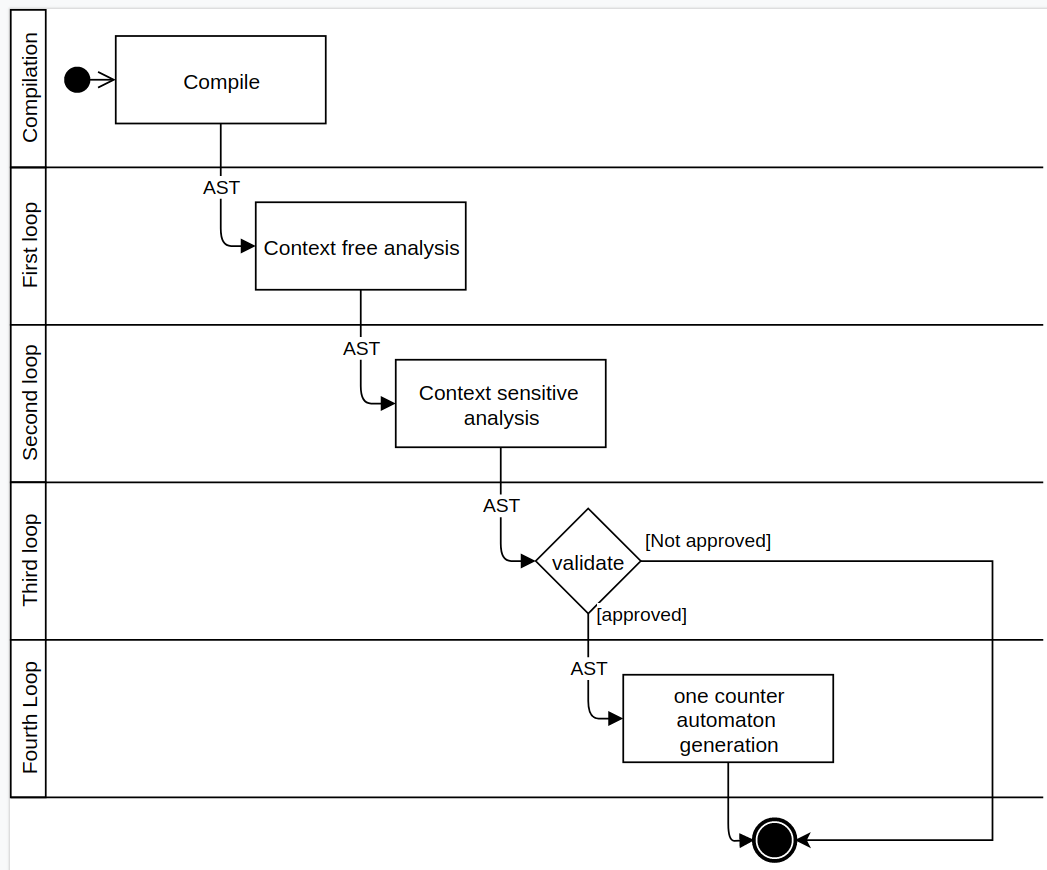
\includegraphics[width=0.75\linewidth]{Images/tool_overview.png}
	\end{figure}
\end{frame}

\section{Related Work}

\begin{frame}{Related work I}
	\begin{biblio}{}
		\biblioref{Daniel Bundala, Joel Ouaknine}{2017}{On parametric timed automata and one-counter machines}{Information and Computation}
		\biblioref{Jérôme Leroux, Grégoie Sutre}{2005}{Flat Counter Automata Almost Everywhere!}{Automated Technology for Verification and Analysis}
		\biblioref{Ahmed Bouajjani, Marius Bozga, Peter Habermehl, Radu Iosif, Pierre Moro, Tomáš Vojnar}{2006}{Programs with Lists Are Counter Automata}{Computer Aided Verification}
	\end{biblio}
\end{frame}

\begin{frame}{Related work II}
	\begin{biblio}{}
		\biblioref{Kravtsev, Makism}{1999}{Quantum Finite One-Counter Automata}{SOFSEM'99: Theory and Practice of Informatics}
	\end{biblio}
\end{frame}

\section{Motivation}

\section{One Counter Automata}

\begin{frame}{Counter automata I}
	\begin{itemize}
		\item Non-Deterministic Finite Automata with counter(s)
		\item limited set of operations
		\begin{itemize}
			\item increment the counter with parameter/constant
			\item compare the counter to parameter/constant
		\end{itemize}
		\item transition relation $\sigma \subseteq Q \times op \times Q$
	\end{itemize}
\end{frame}
\begin{frame}{Counter automata II}
	\begin{figure}[h!]
		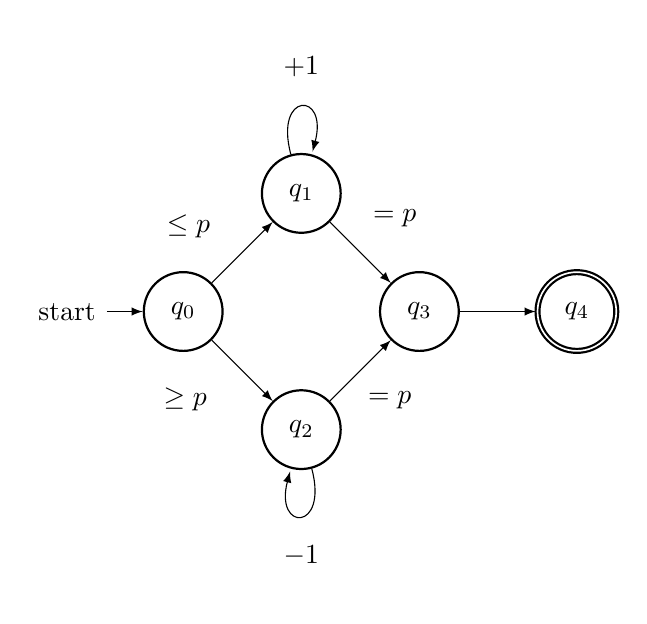
\begin{tikzpicture}[auto, >=latex, node distance = 2 cm, minimum size = 1 cm]
			\tikzstyle{round} = [thick, draw=black, circle]
			
			\node[round, initial] 	at (-1.5, 0) 	(q0) 	{$q_0$};
			\node[round] 			at (0, 1.5) 	(q1) 	{$q_1$};
			\node[round] 			at (0, -1.5) 	(q2) 	{$q_2$};
			\node[round] 			at (1.5, 0) 	(q3) 	{$q_3$};
			\node[round, accepting]	at (3.5, 0)		(q4)	{$q_4$};
				
			\path[->]
			(q0)	edge					node	[xshift = -5pt, yshift=-5pt]	{$\leq p$} 	(q1)
			(q0)	edge 					node 	[xshift=-35pt, yshift=-25pt]	{$\geq p$} 	(q2)
			(q1)	edge	[loop above]	node									{$+1$}		(q1)
			(q2)	edge	[loop below]	node									{$-1$}		(q2)
			(q1)	edge					node	[xshift = -2pt, yshift=-2pt]	{$=p$}		(q3)
			(q2)	edge					node	[xshift=25pt, yshift=-25pt]		{$=p$}		(q3)
			(q3)	edge					node									{$ $}		(q4);
		\end{tikzpicture}
	\end{figure}
\end{frame}


\end{document}
